\section{ДД/Splay}

\subsection{ДД}
Мысленно пронумеруем вершины ДД по возрастанию ключей, получим $v_1, v_2, \ldots, v_n$. Докажем, что мат. ожидание глубины конкретной вершины $v_a$ равно $O(\log n)$. Очевидно, глубина равна количеству предков (не обязательно непосредственных). Пусть индикатор $I_b$ равен 1, если $v_b$ предок $v_a$, и 0 иначе. Чтобы $v_b$ была предком $v_a$, нужно, чтобы приоритеты у вершин $v_i$ для $i \in [a, b)$ были меньше приоритета $v_b$, ведь они обязаны находиться вместе с $v_a$ в поддереве $v_b$, а ДД --- куча по приоритетам. Значит, $E(I_b)$, то есть вероятность того, что $v_b$ предок $v_a$, не больше вероятности того, что среди приоритетов для $v_i, i \in [a, b]$ приоритет у $v_b$ наибольший. Вероятность последнего, очевидно, равна $\frac{1}{|a - b| + 1}$. Значит,
\[
E(\text{глубина }v_a) = \sum_{b = 1}^n E(I_b) \leq \sum_{b = 1}^n \frac{1}{|a - b| + 1} \leq 2 \sum_{s = 1}^{n} \frac{1}{s} = O(\log n)
\]

Так как все операции работают с ДД за $O(\text{глубина какой-то вершины})$, получаем, что хотелось.

\subsection{Splay}
\newcommand{\sz}{\operatorname{sz}}


Повороты выглядят так:
\begin{figure}[htbp]
    \centering
    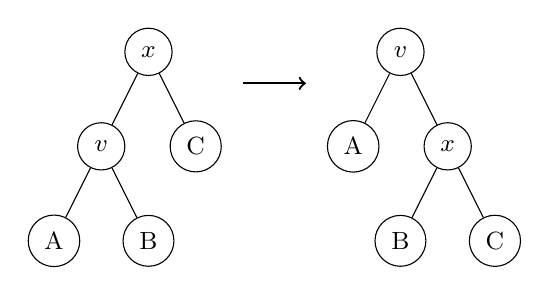
\begin{tikzpicture}[
        level distance=15mm,
        sibling distance=15mm,
        every node/.style={circle, draw, minimum size=6mm, font=\small},
        scale=0.8
    ]
      % Before tree
      \node (x) {$x$}
        child { node (y) {$v$} 
          child { node {A} }
          child { node {B} }
        }
        child { node {C} };
      
      % After tree
      \begin{scope}[xshift=4cm]
        \node (y) {$v$}
          child { node {A} }
          child { node (x) {$x$}
            child { node {B} }
            child { node {C} }
          };
      \end{scope}
      
      % Arrow between trees
      \draw[->, thick] (1.5,-0.5) -- (2.5,-0.5);
    \end{tikzpicture}
    \captionsetup{labelformat=empty}
    \caption{\texttt{zig} (право)}
\end{figure}

\begin{figure}[htbp]
    \centering
    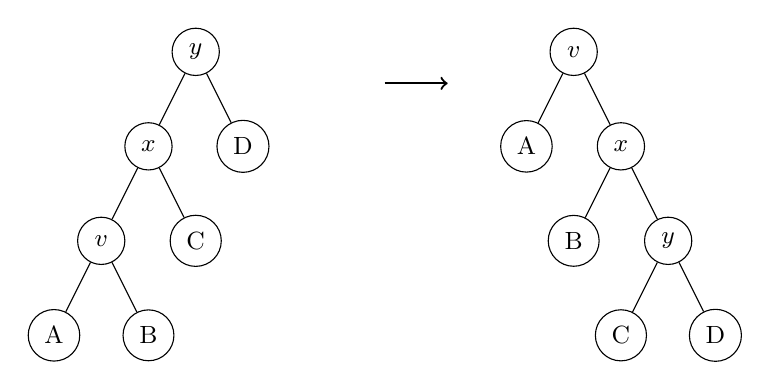
\begin{tikzpicture}[
        level distance=15mm,
        sibling distance=15mm,
        every node/.style={circle, draw, minimum size=6mm, font=\small},
        scale=0.8
    ]
        % Before tree
        \node (z) {$y$}
        child { node (y) {$x$}
            child { node (x) {$v$}
            child { node {A} }
            child { node {B} }
            }
            child { node {C} }
        }
        child { node {D} };
    
        % After tree
        \begin{scope}[xshift=6cm]
        \node (x) {$v$}
            child { node {A} }
            child { node (y) {$x$}
            child { node {B} }
            child { node (z) {$y$}
                child { node {C} }
                child { node {D} }
            }
            };
        \end{scope}
        
        % Arrow between trees
        \draw[->, thick] (3,-0.5) -- (4,-0.5);
    \end{tikzpicture}
    \captionsetup{labelformat=empty}
    \caption{\texttt{zig-zig} (право-право)}
\end{figure}

\begin{figure}[htbp]
    \centering
    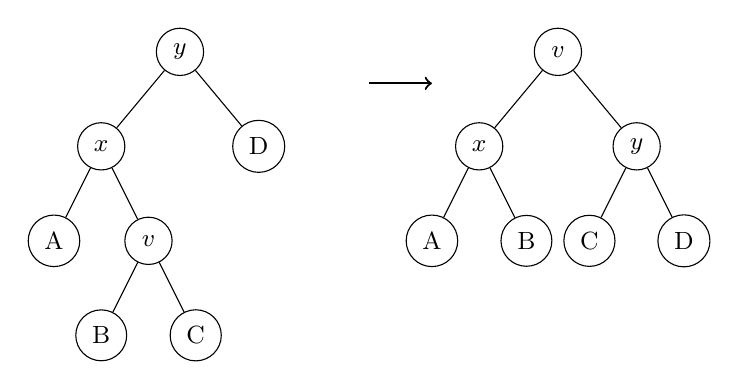
\begin{tikzpicture}[
        level distance=15mm,
        sibling distance=25mm,
        every node/.style={circle, draw, minimum size=6mm, font=\small},
        scale=0.8
    ]
      % Исходное дерево
      \node (z) {$y$}
        child { node (y) {$x$} [sibling distance=15mm]
          child { node {A} }
          child { node (x) {$v$}
            child { node {B} }
            child { node {C} }
          }
        }
        child { node {D} };
    
      % Исправленное правое дерево
      \begin{scope}[xshift=6cm]
        \node (x) {$v$}
          child { node (y) {$x$} [sibling distance=15mm]
            child { node {A} }
            child { node {B} }
          }
          child { node (z) {$y$} [sibling distance=15mm] % <-- Изменено здесь
            child { node {C} }
            child { node {D} }
          };
      \end{scope}
      
      % Стрелка между деревьями
      \draw[->, thick] (3,-0.5) -- (4,-0.5);
    \end{tikzpicture}
    \caption{\texttt{zig-zag} (право-лево)}
\end{figure}


Докажем, что амортизированное время работы \texttt{splay}($v$) равно $O(\log n)$. Сделаем это методом потенциалов. Пусть $r(v) = \log \sz(v)$, где $\sz(v)$ --- размер поддерева вершины $v$ (здесь и везде далее под $\log$ понимается двоичный логарифм). Потенциал $\Phi = \sum\limits_{v} r(v)$. Очевидно, что $0 \leq \Phi \leq n \log_2 n$.

\begin{statement}
$t_i + \Delta \Phi \leq 1 + 3(r(root) - r(v))$, где $t_i$ --- время работы.
\end{statement}
\underline{Доказательство}: сначала отдельно оценим изменение потенциала при выполнении одного \texttt{zig}, \texttt{zig-zig} или \texttt{zig-zag}
\begin{enumerate}
    \item \texttt{zig}. Пусть без ограничения общности делали правый поворот (как на рисунке). Хотим доказать, что $t_\texttt{zig} + \Delta \Phi \leq 1 + 3(r(x) - r(v))$. Повороты делаются за $O(1)$, поэтому будем считать $t_\texttt{zig} = 1$. Значит, нужно нужно доказать, что 
    \[ 1 + \cancel{\log(A + B + C + 2)} + \log(B + C + 1) - \cancel{\log(A + B + C + 2)} - \bcancel{\log(A + B + 1)} \leq 
    \] \[ \leq 1 + 3 \log(A + B + C + 2) - \bcancel{3\log(A + B + 1)} \]
    \[ \impliedby \log(B + C + 1) + 2 \log(A + B + 1) \leq 3 \log(A + B + C + 2) \]


    А последнее, очевидно, верно.

    \item \texttt{zig-zig}. Пусть без ограничения общности делали правый-правый поворты (как на рисунке). Хотим доказать, что $t_\texttt{zig-zig} + \Delta \Phi \leq 3(r(y) - r(v))$, то есть
    \[ 1 + \cancel{\log(A + B + C + D + 3)} + \log(B + C + D + 2) + \log(C + D + 1) - \cancel{\log(A + B + C + D + 3)} - \]
    \[ -\log(A + B + C + 2) - \bcancel{\log(A + B + 1)} \leq 3\log(A + B + C + D + 3) - \bcancel{3\log(A + B + 1)} \]
    \[ \impliedby 1 + \cancel{\log(B + C + D + 2)} + \log(C + D + 1) + \bcancel{2 \log(A + B + 1)} \leq \cancel{3\log(A + B + C + D + 3)} + \bcancel{\log(A + B + C + 2)}\]
    \[ \impliedby 1 + \log(C + D + 1) + \log(A + B + 1) \leq 2\log(A + B + C + D + 3) \]

    Пусть $a = C + D + 1, b = A + B + 1$. Докажем, что $1 + \log a + \log b \leq 2\log (a + b)$, из этого будет следовать требуемое. 
    \[ 1 + \log a + \log b \leq 2 \log(a + b) \]
    \[ 1 \leq \log((a + b)^2) - \log ab \]
    \[ 1 \leq \log \frac{a^2 + 2ab + b^2}{ab} \]
    \[ 1 \leq \log (2 + ...) \]

    Последнее верно, так как логирфм двоичный и $... \geq 0$.

    \item \texttt{zig-zag}. Пусть без ограничения общности делали правый-левый поворты (как на рисунке). Хотим доказать, что $t_\texttt{zig-zag} + \Delta \Phi \leq 3(r(y) - r(v))$, то есть
    \[ 1 + \cancel{\log(A + B + C + D + 3)} + \log(A + B + 1) + \log(C + D + 1) - \cancel{\log(A + B + C + D + 3)} - 
    \] \[  - \log(A + B + C + 2) - \bcancel{\log(B + C + 1)} \leq 3\log(A + B + C + D + 3) - \bcancel{3\log(B + C + 1)} \]
    \[ \impliedby 1 + \log(A + B + 1) + \log(C + D + 1) + \xcancel{2 \log(B + C + 1)} \leq \cancel{3\log(A + B + C + D + 3)} + \bcancel{\log(A + B + C + 2)} \]
    \[ \impliedby 1 + \log(A + B + 1) + \log(C + D + 1) \leq 2\log(A + B + C + D + 3) \]

    Что, как уже доказывалось ранее, верно.
\end{enumerate}

Пусть во время $\texttt{splay}(v_0)$ на пути до $v_0$ были вершины $v_k = root, v_{k - 1}, \ldots, v_0$. Тогда суммарное время работы $t_i$ равно сумме времён работ всех $t_\texttt{zig}, t_\texttt{zig-zig}, t_\texttt{zig-zag}$. Она, если идти снизу вверх, оценивается как $\leq 1 + 3(r(v_2) - r(v^{(0)}_0)) + 3(r(v_4) - r(v^{(1)}_0)) + \ldots + 3(r(v_k) - r(v^{(s)}_0))$, где $v^{(i)}_0$ вершина $v_0$ поднятая $i$ раз, то есть прошедшая $i$ операций. Но заметим, что, после подъёма $v^{(i)}_0$ размер её поддерева становится таким же, какой был у предыдущего корня соответствующего поддерева. Значит, эта сумма просто равна $1 + 3(r(v_2) - r(v_0)) + 3(r(v_4) - r(v_2)) + \ldots + 3(r(v_k) - r(v_{k - (\text{1 или 2})})) = 1 + 3(r(root) - r(v))$ $\blacksquare$
\let\sz\undefined

\bigskip

Так как $1 + 3(r(root) - r(v)) = O(\log n)$, по методу потенциалов получаем, что амортизированное время работы \texttt{splay}($v$) равно $O(\log n)$.

Теперь хотим научить делать что-то более содержательное. Так, допустим, хотим сделать \texttt{find}/\texttt{lower\_bound} по ключу. Честно спустимся по дереву как по бинарному дереву поиска, а потом от конечной вершины запустим \texttt{splay}. Время, затраченное на спуск, будет равно времени, затраченному на \texttt{splay}, которое амортизированно $O(\log n)$. Научимся делать \texttt{split} от вершины $v$. Просто делаем $\texttt{splay}(v)$, левое поддерево $v$ и $v$ вместе с правым поддеревом --- результат \texttt{split}, от такого потенциал только уменьшится. Для того, чтобы делать \texttt{split} по значению, сначала делаем \texttt{lower\_bound}, потом \texttt{split}. Если надо делать \texttt{merge}, можно для первого (т.е. меньшего по ключам) дерева поднять самую правую вершину, а затем к ней подвесить второе дерево как правого сына. От этого потенциал увеличится на не более чем $\log n$, что допустимо для метода потенциалов. \texttt{insert}/\texttt{erase} очевидно делаются через все операции выше, также изменяют потенциал на не более чем $\log_2(n)$.